%-----------------------------------------------------------------------------
%
%               Template for sigplanconf LaTeX Class
%
% Name:         sigplanconf-template.tex
%
% Purpose:      A template for sigplanconf.cls, which is a LaTeX 2e class
%               file for SIGPLAN conference proceedings.
%
% Guide:        Refer to "Author's Guide to the ACM SIGPLAN Class,"
%               sigplanconf-guide.pdf
%
% Author:       Paul C. Anagnostopoulos
%               Windfall Software
%               978 371-2316
%               paul@windfall.com
%
% Created:      15 February 2005
%
%-----------------------------------------------------------------------------


\documentclass{sigplanconf}

% The following \documentclass options may be useful:

% preprint      Remove this option only once the paper is in final form.
% 10pt          To set in 10-point type instead of 9-point.
% 11pt          To set in 11-point type instead of 9-point.
% authoryear    To obtain author/year citation style instead of numeric.

\usepackage{amsmath}

\usepackage{graphicx}
\graphicspath{ {images/} } % Path to images folder

\begin{document}

\special{papersize=8.5in,11in}
\setlength{\pdfpageheight}{\paperheight}
\setlength{\pdfpagewidth}{\paperwidth}

\conferenceinfo{CONF '14}{September 29, 2014, 2014, Golden, CO, USA} 
\copyrightyear{2014} 
\copyrightdata{978-1-nnnn-nnnn-n/yy/mm} 
\doi{nnnnnnn.nnnnnnn}

% Uncomment one of the following two, if you are not going for the 
% traditional copyright transfer agreement.

%\exclusivelicense                % ACM gets exclusive license to publish, 
                                  % you retain copyright

%\permissiontopublish             % ACM gets nonexclusive license to publish
                                  % (paid open-access papers, 
                                  % short abstracts)

\titlebanner{banner above paper title}        % These are ignored unless
\preprintfooter{short description of paper}   % 'preprint' option specified.

\title{GPU-Based Parallel Finite State Machines}

\authorinfo{Kameron W. Kincade\and Ryan P. Langewisch}
           {Colorado School of Mines}
           {kkincade@mines.edu | rlangewi@mines.edu}

\maketitle

\begin{abstract}
Abstract goes here.
\end{abstract}

% general terms are not compulsory anymore, 
% you may leave them out
\terms
finite state machines, GPU, parallelization

\section{Introduction}

A finite state machine (FSM) is used to represent an object that can exist in a limited number of states and that can change state based on a number of well-defined rules (Figure 1). Each FSM is responsible for processing various inputs (each usually represented as a string of characters) and determining if these inputs satisfy the machine's acceptance criteria, such as ending in a correct final state. To operate on an input string, the FSM begins with the start state (A in Figure 1) and processes each character one after another. The state machine's rules, along with the input character, dictate the next location to move to. An acceptance state (D) is commonly indicated by a double circle and represents a valid input solution that satisfies the FSM's criteria.

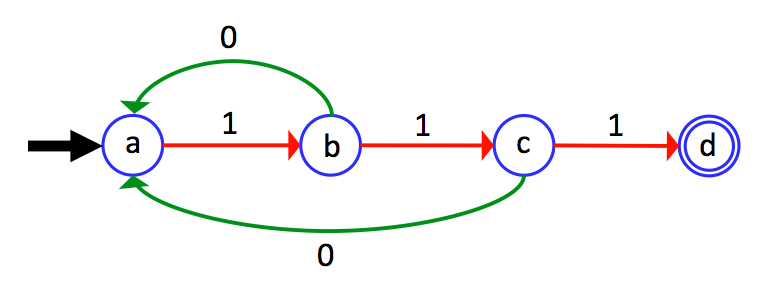
\includegraphics[width=\linewidth]{fsm_diagram.png}

FSMs are embedded in many different types of applications, including web application computations, such as lexing, parsing, translations, and media encoding/decoding. With the recent emphasis on mobile, handheld devices, the need for a computationally efficient implementation of FSMs is becoming more important. Parallelization is one of the obvious ways to speed up the execution of a program. However, the simple structure and procedures of a FSM also make them difficult to parallelize. The most evident way to parallelize a FSM is to divide the input string into a number of different FSM input strings, each of which can be processed in parallel. The problem with this approach is determining the start state for each new input string. The start state of one input string should be the end state of the previous input string, but this can't be calculated in advanced for

Lots of text.

More text.

Lots of text.

More text.


Lots of text.

More text.

Lots of text.

More text.


Lots of text.

More text.

Lots of text.

More text.

Lots of text.

More text.

Lots of text.

More text.

Lots of text.

More text.

Lots of text.

More text.

Lots of text.

More text.

Lots of text.

More text.

Lots of text.

More text.

Lots of text.

More text.


Lots of text.

More text.

Lots of text.

More text.


Lots of text.

More text.

Lots of text.

More text.

Lots of text.

More text.

Lots of text.

More text.

Lots of text.

More text.

Lots of text.

More text.

Lots of text.

More text.

Lots of text.

More text.


Lots of text.

More text.

Lots of text.

More text.




Lots of text.

More text.

Lots of text.

More text.

Lots of text.


Lots of text.

More text.

Lots of text.

More text.

Lots of text.

More text.

Lots of text.

More text.

Lots of text.

More text.

Lots of text.

More text.

Lots of text.

More text.

Lots of text.

More text.

Lots of text.

More text.

Lots of text.

More text.

Lots of text.

More text.

Lots of text.

More text.

Lots of text.

\appendix
\section{Appendix Title}

This is the text of the appendix, if you need one.

\acks

Acknowledgments, if needed.

% We recommend abbrvnat bibliography style.

\bibliographystyle{abbrvnat}

% The bibliography should be embedded for final submission.

\begin{thebibliography}{}
\softraggedright

\bibitem[Smith et~al.(2009)Smith, Jones]{smith02}
P. Q. Smith, and X. Y. Jones. ...reference text...

\end{thebibliography}


\end{document}

%                       Revision History
%                       -------- -------
%  Date         Person  Ver.    Change
%  ----         ------  ----    ------

%  2013.06.29   TU      0.1--4  comments on permission/copyright notices

